\documentclass{article}

% --- load packages ---

\usepackage[margin=1in]{geometry} % change the margins
\usepackage{amsmath} % useful math environments and commands like align
\usepackage{amssymb} % assumes amsmath package installed
\usepackage[colorlinks,bookmarks,bookmarksnumbered,allcolors=blue]{hyperref} % hyperlinks between references
\usepackage{graphicx}  % include images
\usepackage[caption=false]{subfig} % subfigures.  false option prevents conflicts in caption styling with other packages
\usepackage{booktabs} % better tables
\usepackage[capitalise]{cleveref} % better referencing. uses cref.
\usepackage[section]{placeins} % sometimes useful to prevent figures from floating out of a section
\usepackage{cite} % handles multiple citations in one command better
\usepackage{doi} % allow correct hypderlinking of DOIs
\usepackage{hyperref}
\usepackage[title]{appendix}
\usepackage{pgfplots}
\usepackage{algorithm} % for algorithm figure
\usepackage{algpseudocode} % for algorithm figure

\usepackage{aircraftshapes}

\newcommand{\norm}[1]{\left\Vert{#1}\right\Vert}
\newcommand{\skewm}[1]{\left[{#1}\right]_{\times}}


\begin{document}

\title{Homework 5}
\author{Jaron Ellingson}
% put in \date{} if you don't want a date to appear, or enter a specific date, otherwise default is today's date.
\maketitle

 %\href{https://byu.box.com/shared/static/anxheci3eytucrh3ke57k2sqdx0ivmjg.pdf}{homework pdf}

\section*{Introduction}

To explore gradient free optimization, I choose to implement a more complex version of my final project. My project is to create a evolutionary nonlinear model predictive control for a fixed wing aircraft. This assignment allowed me to make big improvement on my project. I will first explain a little about model predictive control and then will highlight how I choose to implement my evolutionary algorithm. I will then compare the Nelder-Mead gradient free method as well as two gradient based methods against my evolutionary algorithm. Finally, I will discuss results on increasing the dimensionality of the Rosenbrock function with gradient-free and gradient based methods.


\section*{Nonlinear Model Predictive Control}

The nonlinear model predictive control (NMPC) problem we want to solve is formulated by

\begin{equation}
\label{eq:objective}
\begin{aligned}
\text{minimizing} & \quad J= \sum_{k=0}^{T-1} (f(\mathbf{x}_k,\mathbf{u}_k)-\mathbf{x}_{d})^{\top} Q (f(\mathbf{x}_k,\mathbf{u}_k)-\mathbf{x}_{d}) \\
\text{with respect to} & \quad \mathbf{u}_k =\begin{bmatrix}s_{a} & s_{e} & s_{t} & s_{r}\end{bmatrix}^{\top} \\
\text{subject to} & \quad -2 \le s_{a} \le 2, \\
& \quad -2 \le s_{e} \le 2, \\
& \quad \hspace{13pt} 0 \le s_{t} \le 1, \\
& \quad -2 \le s_{r} \le 2,
\end{aligned}
\end{equation}

where $f(\mathbf{x}_k,\mathbf{u}_k)$ represents the nonlinear dynamics of a fixed wing aircraft applied with Runge-Kutta 4th order approximation (see Appendix \ref{sec:dynamics} for more details). $\mathbf{x}_k$ and $\mathbf{x}_{d}$ are our calculated state and desired state where,

\begin{equation}
\label{eq:lqr_current_desired_states}
\mathbf{x}=\begin{bmatrix}\mathbf{p} \\ \mathbf{v} \\ \mathbf{q} \\ \boldsymbol{\omega}\end{bmatrix}.
\end{equation}

Furthermore, $Q$ is our cost matrix and initialized as,

\begin{equation}
Q = \text{diagonal}(\begin{bmatrix}
	0,0,100,1,0,0,50,50,50,0,0,0
\end{bmatrix}).
\end{equation}

I choose this particular cost because I don't necessarily want the aircraft to hit a particular location but to maintain a desired altitude and heading while also maintaining a desired forward velocity. This can be seen in \Cref{fig:vet_field} where the aircraft is some distance away from the the direct path from $w_{i-1}$ to $w_i$. \Cref{fig:vet_field} also shows a vector field which slowly places the aircraft onto a course to the next waypoint. This vector field allows us to define the commanded heading of the aircraft as we are far away from the desired path. this vector field is defined as,

\begin{equation}
\check{\chi}=\chi_{l}-\chi_{\infty}\frac{2}{\pi}\tan^{-1}\left(k_{\chi}\mathbf{e}_{2}\right),
\end{equation}

where $\chi_l$ is the course angle of our line, and $\check{\chi}$ is the desired course angle. Furthermore, $k_\chi$ is a positive gain and $\chi_\infty$ is the maximum allowed difference between $\check{\chi}$ and $\chi_l$.

%\begin{figure}
%	\centering
%	\begin{tikzpicture}
%	\coordinate[label = above right:$w_{i}$] (wi) at (2,3);
%	\node at (wi)[circle,fill,inner sep=2.5pt]{};
%	\coordinate[label = above left:$w_{i-1}$] (wi1) at (-2,0);
%	\node at (wi1)[circle,fill,inner sep=2.5pt]{};
%	\draw (wi1) -- (wi);
%	\draw [densely dotted] plot [smooth, tension=1] coordinates {(0,0) (-0.25,1.05) (0.5,1.85)};
%	\node [aircraft top,fill=black,minimum width=0.75cm,rotate=120] at (0,0) {};
%	\end{tikzpicture}
%	\caption{Waypoint Picture.}
%	\label{fig:fw_waypoints}	
%\end{figure}

\begin{figure}
	\centering
	\begin{tikzpicture}
	\def\length{sqrt(1+(-pi/6*2/pi * atan(0.1*x))^2)}
	\begin{axis}[
	title={},
	domain=-2:2,
	view={0}{90},
	axis background/.style={fill=white},
	xticklabels={},
	yticklabels={},
	ticks=none,
	]
	\addplot3[black,
	quiver={
		u={-pi/6*2/pi * atan(0.1*x)/\length},
		v={1/\length},
		scale arrows=0.3,
	},
	-stealth,samples=15]
	{x};
	\end{axis}
	%\draw [very thick][-latex](160pt,20pt)..controls(100pt,25pt) and (60pt,45pt)..(42pt,58pt);
	%\filldraw(160pt,20pt)circle(2pt) (100pt,25pt)circle (2pt) (60pt,45pt)circle (2pt) (42pt,58pt)circle (2pt);
	\coordinate[label = above:$w_{i}$] (wi) at (97.5pt,161pt);
	\node at (wi)[circle,fill,inner sep=2.5pt]{};
	\coordinate[label = below:$w_{i-1}$] (wi1) at (97.5pt,0pt);
	\node at (wi1)[circle,fill,inner sep=2.5pt]{};
	\draw[very thick] (wi1) -- (wi);
	
	\draw [line width=2pt, dash pattern=on \pgflinewidth off 2pt] plot [smooth, tension=0.75] coordinates {(140pt,37pt) (105pt,60pt) (97.5pt,100pt)};
	\node [aircraft top,fill=black,minimum width=0.75cm,rotate=160] at (150pt,33.5pt) {};
	
	%\filldraw(97.5pt,161pt)circle(2pt) (97.5pt,0pt)circle(2pt);
	%\draw[very thick] (97.5pt,161pt) -- (97.5pt,0pt);
	\end{tikzpicture}
	\caption{A vector field which converges onto a path from one waypoint to another.}
\label{fig:vet_field}

\end{figure}

My design variables $\mathbf{u}_k =\begin{bmatrix}s_{a} & s_{e} & s_{t} & s_{r}\end{bmatrix}^{\top}$ represent the control inputs to the system and are constrained to be within certain bounds. The aileron, elevator, and rudder are all constrained to be within -2 to 2 radians and the throttle is constrained from 0 to 1. To reduce the number of design variables, I choose to have the inputs applied along a segment of the trajectory and do not choose a new input at every time step. I choose to have 10 control inputs for a time horizon of 1 second with time steps of 0.01 seconds. This means every 0.1 seconds I apply a new control input. \Cref{fig:sub2,fig:cd2} shows only 10 inputs applies over the trajectory of 1 second for two separate test cases.

\section*{Evolutionary Algorithm}

The evolutionary algorithm has 4 major components: fitness, selection, crossover, and mutation. The fitness is described above as the objective function. The other components will be described here in detail.

\subsection*{Selection}

I choose to implement a population which has $n$ number of individuals with $m$ number of parents. These parents are the only individuals which are allowed into the mating phase and are the only individuals allowed to continue into the next generation with no changes. The parents are selected by being the best $m$ individuals at every generation. This allows for the best individuals to carry on from generation to generation. For these results I choose to have $n=50$ and $m=5$.

\subsection*{Crossover}

The crossover scheme created a new population based on only the parents from the previous generation. I randomly choose two different parents and assigned their child to randomly received an input from either parent for each input $s_{a}, s_{e}, s_{t}, s_{r}$ at a randomly location in the trajectory. Overall I had to generate $n-m-s$ children at every generation (see what $s$ is below).

\subsection*{Mutation}

I didn't allow for mutation to happen on individual inputs for each child in this simulation but I have implemented the structure to randomly insert noise onto the children if I decide to test this for the final project. I also allowed for a certain number $s$ of strangers to be inserted into the population with randomly generated trajectories. This allowed for the population to avoid becoming stagnant. 

Finally, I restricted the number of generations for the population to crossover and mutate to be 100 generations. I choose to limit the algorithm in this way to increase the speed at which we can generate estimated inputs to maintain our trajectory.

\section*{Results}

I will now compare the four methods for solving the optimization (\cref{eq:objective}). These results will compare a single optimization over one trajectory. Typically we will want to resolve this optimization at every time step. The desired states for each test case are show by

\begin{equation}
x_{d1}=
\begin{bmatrix}
	0 \\ 0 \\ -100 \\ 15 \\ 0 \\ 0 \\ 0 \\ 0 \\ 0 \\ 0 \\ 0 \\ 0 \\
\end{bmatrix},  \quad
x_{d2}=
\begin{bmatrix}
0 \\ 0 \\ -100 \\ 15 \\ 0 \\ 0 \\ 0.7854 \\ 0 \\ 1.5708 \\ 0 \\ 0 \\ 0 \\
\end{bmatrix}, 
\end{equation}

where $x_{d1}$ is the desired state for case 1 and $x_{d2}$ is the desired state for case 2. Notice that I don't command a desired positions except for an altitude and only a forward velocity. This is because I only really care about the heading in the right direction. For case 2 I also commanded a 45 deg roll so that the aircraft can continue to turn once we solve for additional time steps.


\Cref{fig:bc,fig:commanded_dir} show the results of the test cases. The first case (\cref{fig:bc}) shows the aircraft already on the commanded heading while the second (\cref{fig:commanded_dir}) shows the aircraft being commanded to perform a 90 deg turn to the right. All four algorithms produce similar visual responses. Notice, however, that the two gradient based methods are able to turn a little more sharply than the gradient-free methods (\cref{fig:cd1}). Additionally, all of the methods appear to have large differences for the inputs (\cref{fig:sub2,fig:cd2}). This indicates that there are possibly many solutions or many inputs which yield similar results.





\begin{figure}[htbp]
	\centering
	\subfloat[]{
		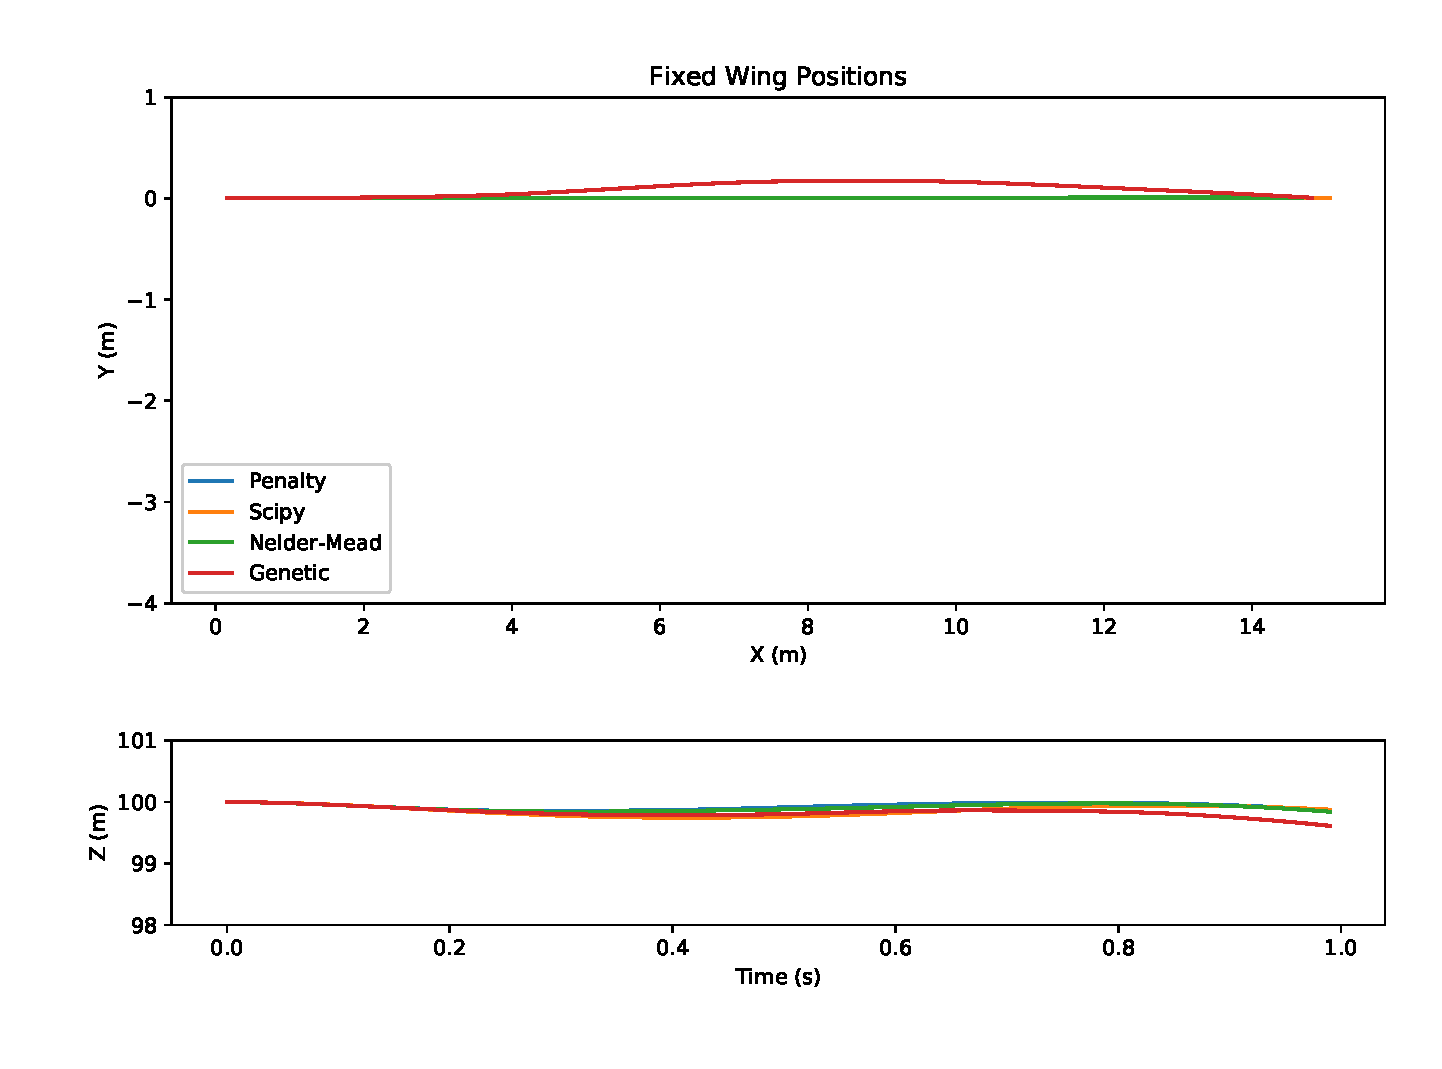
\includegraphics[width=0.45\textwidth]{figures/positions1.eps}
		\label{fig:sub1}
	}
	\qquad
	\subfloat[]{
		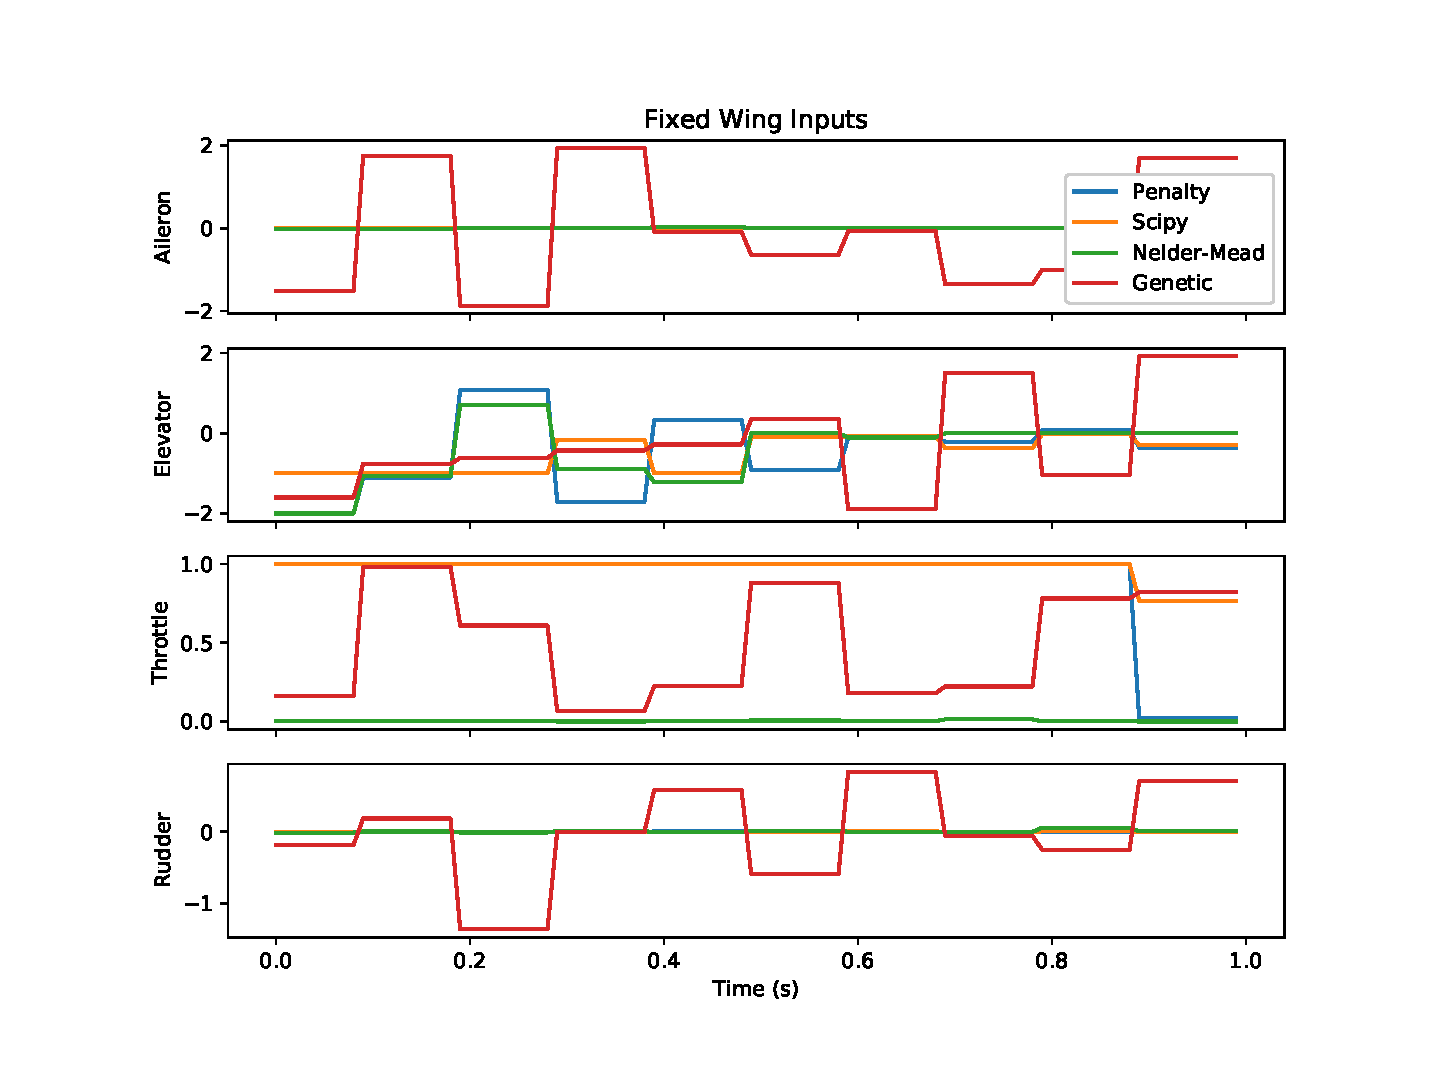
\includegraphics[width=0.45\textwidth]{figures/inputs1.eps}
		\label{fig:sub2}
	}
	\caption{Case 1 is a base case to see if the optimization knows how to keep the aircraft in level flight.}
	\label{fig:bc}
\end{figure}


\begin{figure}[htbp]
	\centering
	\subfloat[]{
		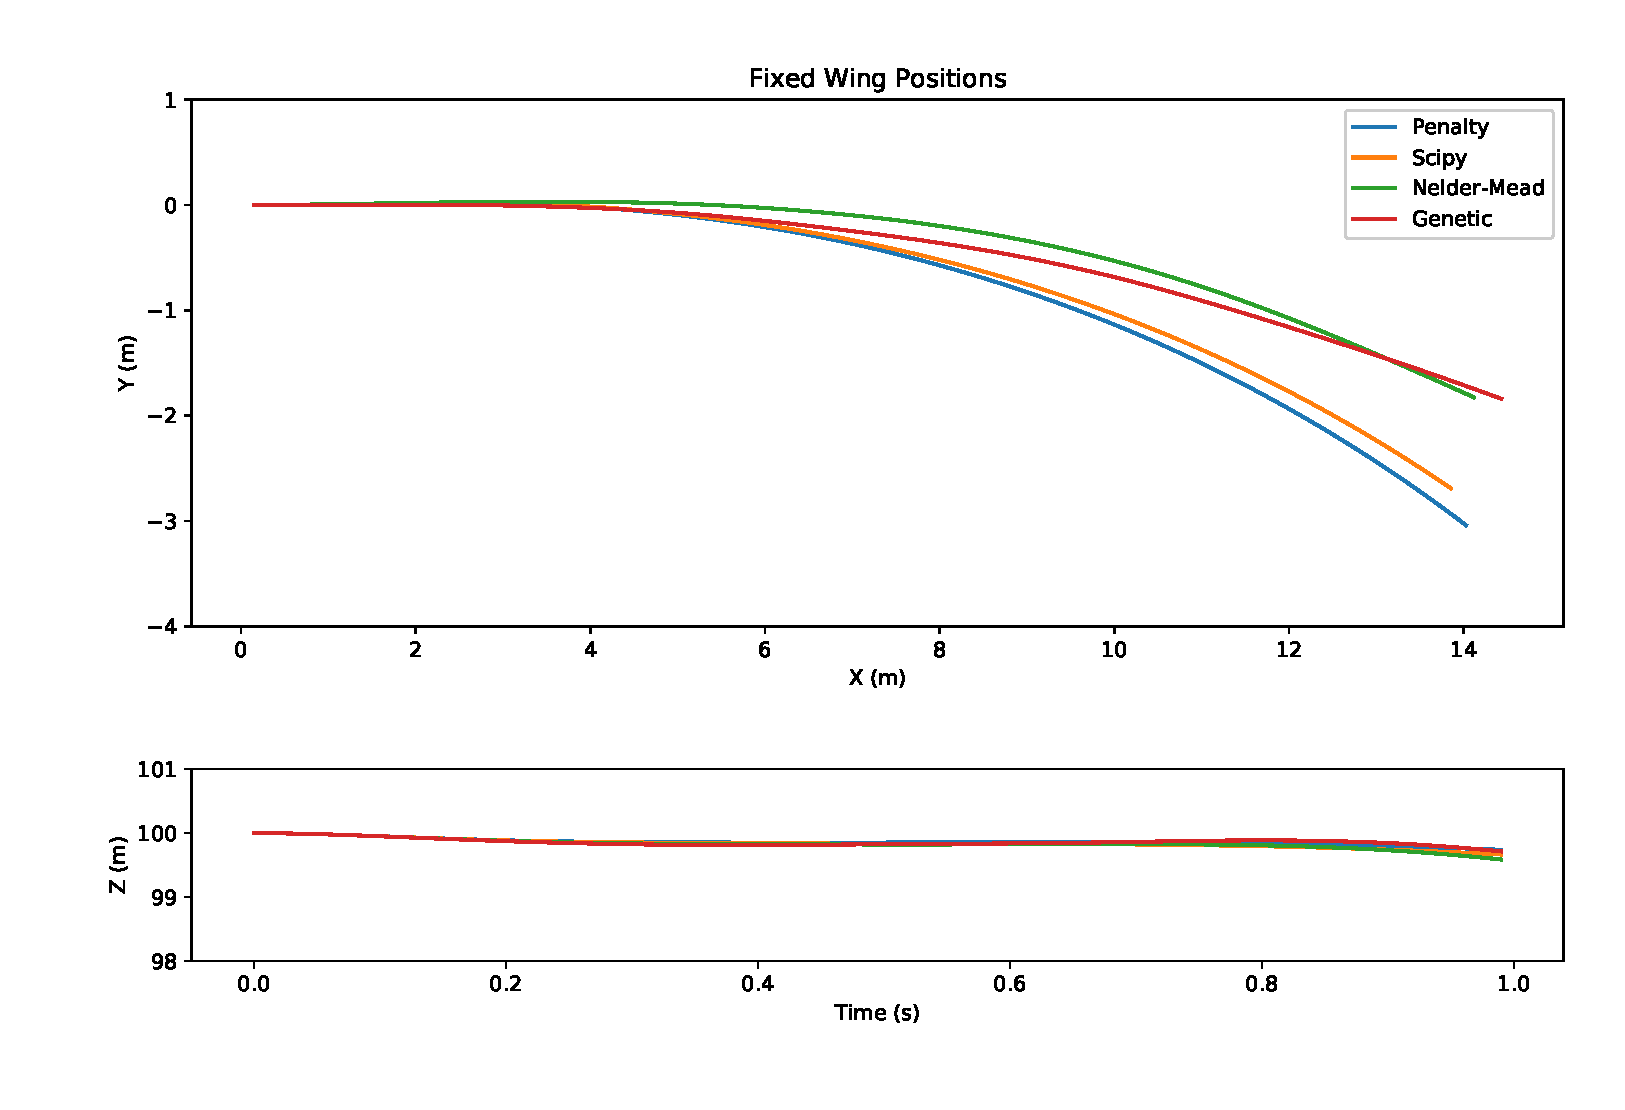
\includegraphics[width=0.45\textwidth]{figures/positions2.eps}
		\label{fig:cd1}
	}
	\qquad
	\subfloat[]{
		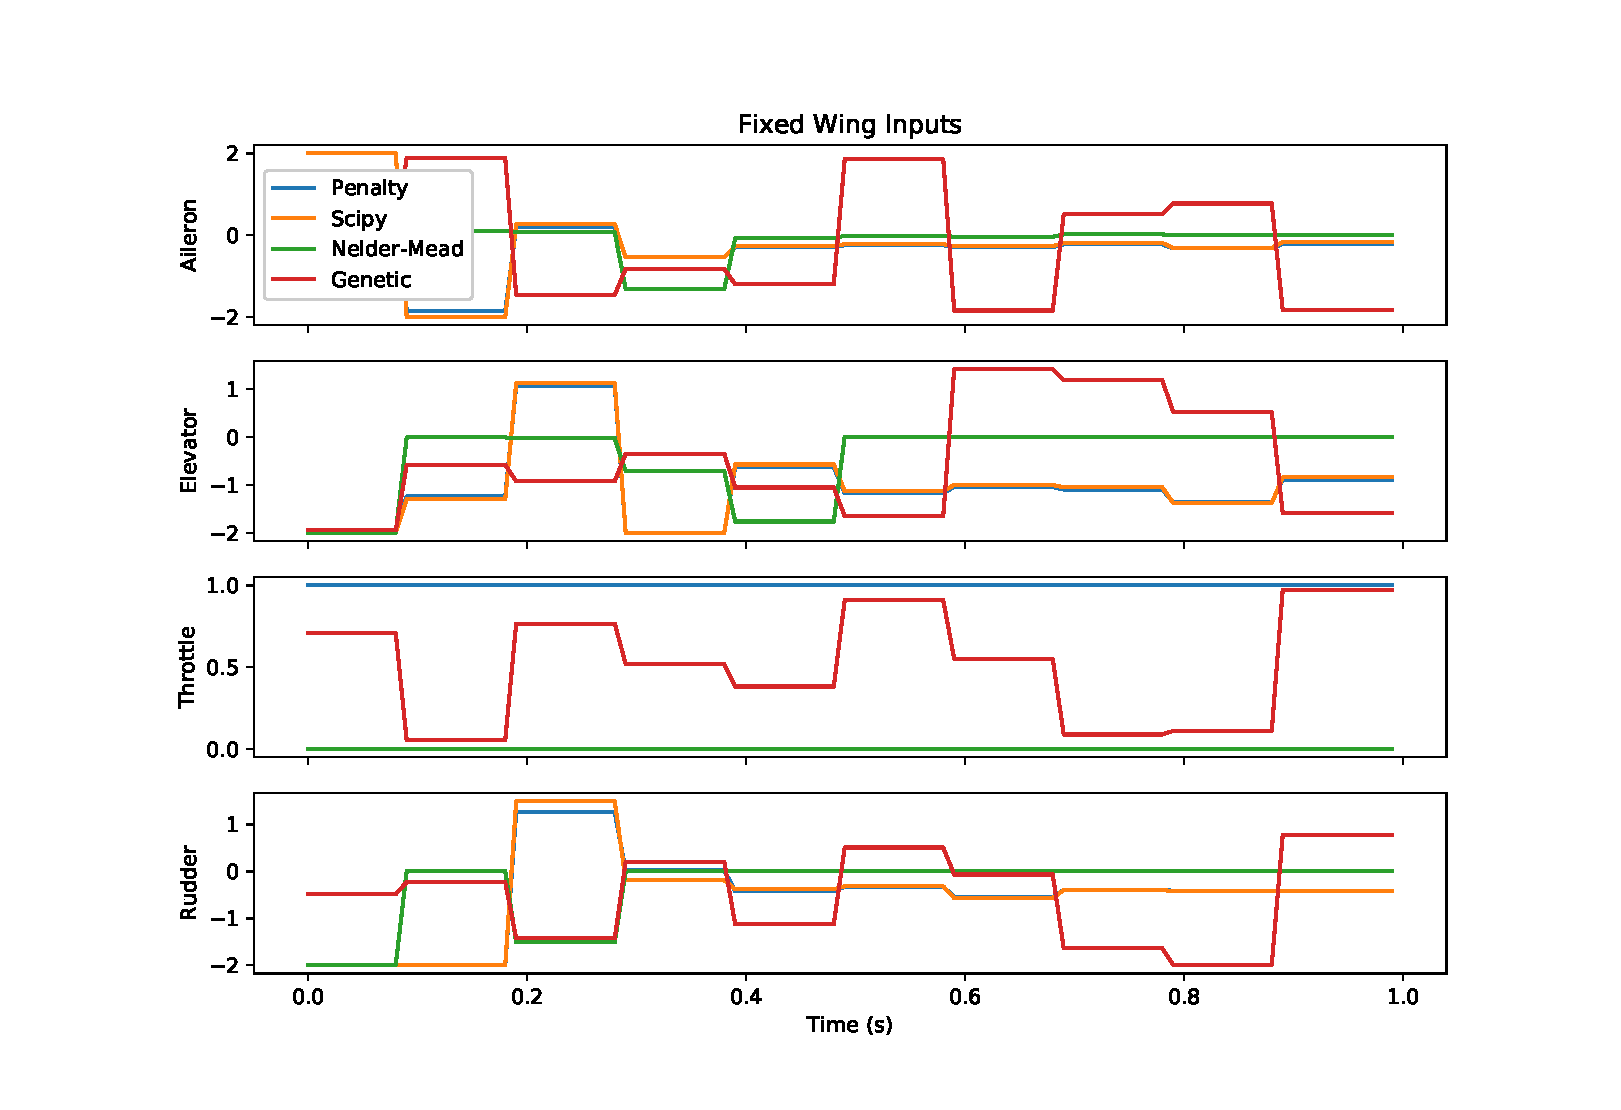
\includegraphics[width=0.45\textwidth]{figures/inputs2.eps}
		\label{fig:cd2}
	}
	\caption{Case 2 tests the aircraft's ability to turn 90 degrees.}
	\label{fig:commanded_dir}
\end{figure}

\Cref{tab:comp_der} further compares the convergence of the four methods. The evolutionary method is able to perform the quickest at 11.001 seconds while Nelder-Mead (NM) with the penalty method takes over 2400 seconds. The last two gradient-base methods also take well over 11 seconds. Also notice that even though the gradient methods appear to visually make a sharper turn (\Cref{fig:cd1}), they do not have the lowest trajectory error nor the final state errors. The evolutionary method appears to be the best choice overall because it does not require a long time to solve and has the best overall trajectory error. We hope to further reduce the solve time to allow for real time solving of the optimization for every time step.

 
\begin{table}[htb]
	\centering
	\caption{We measured convergence efficiency of the four mentioned algorithms through comparing solve time, total trajectory error, and final state error.}
	\label{tab:comp_der}
	\begin{tabular}{c|c|c|c}
		\toprule
		Algorithm & Solve Time (s) & Total Trajectory Error & Final State Error\\
		\midrule
		EMPC & 11.001 & 435.704 & 16.619 \\
		Penalty - NM & $>$ 2400 & 455.015 & 9.906 \\
		Penalty - SLSQP & 811.865 &  547.245 & 11.057 \\
		Scipy - SLSQP  & 124.505 & 543.883 & 11.458 \\
		\bottomrule
	\end{tabular}
\end{table}



\section*{Increasing Dimensionality}

The last task of this assignment was to explore increasing the dimensionality of the Rosenbrock function,

$$ f(x) = \sum_{n-1}^{i} (100(x_{i+1}-x_i^2)^2+(1-x_i)^2). $$ 

I implemented three different approaches to solving this problem. This first was a gradient-free method called the Nelder-Mead algorithm. The second was implementing a finite-difference method and the third was implementing the exact gradients. \Cref{fig:dimensionality} shows how each method increased with function calls as the number of variables increases. The Nelder-Mead takes an astounding 10000x the number of function calls for 64 variables when compared to using the exact gradients. 

Finally, each of the methods were checked to see if they optimized to the correct solution. \Cref{tab:dimensionality} shows the average L2 norm of the difference between the optimal solution of 1 and what the different approaches produced as the final solution. Each method arrived at a optimal solution for each case.


\begin{figure}[htbp]
	\centering
	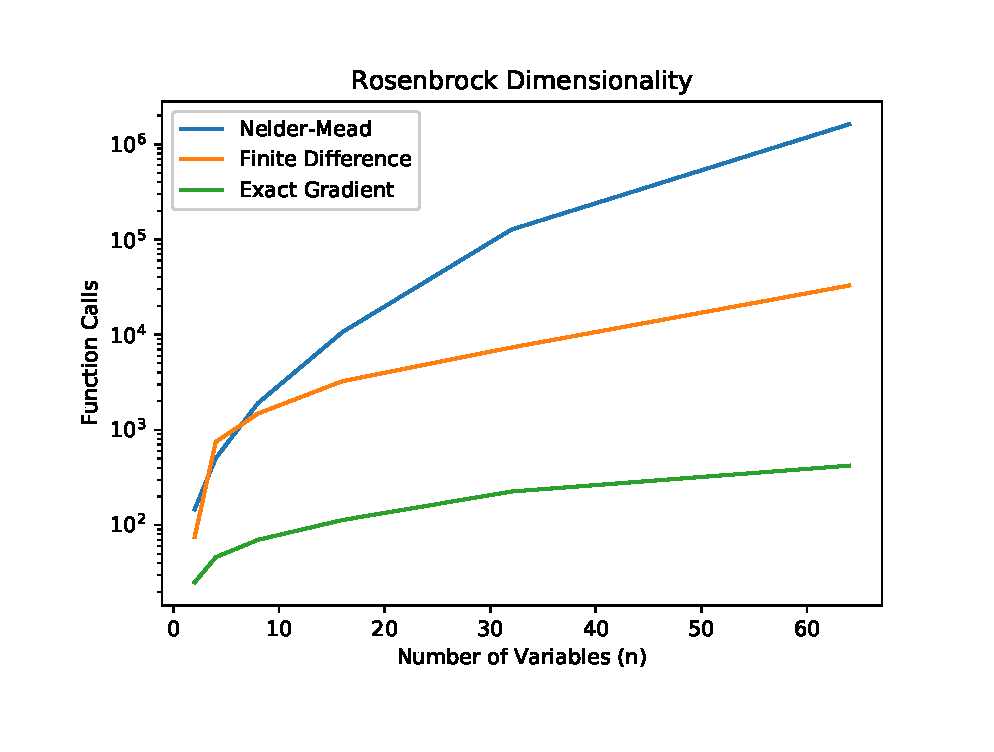
\includegraphics[width=0.6\textwidth]{figures/dimensionality.eps}
	\caption{The dimensionality of the Rosenbrock function with points 2,4,8,16,32,64. This plot compares the Nelder-Mead, finite-difference gradients, and exact gradients as a function of how many design variables are used.}
	\label{fig:dimensionality}
\end{figure}

\begin{table}[htb]
	\centering
	\caption{The average error of each of the approached to the Rosenbrock. They all optimize to the correct solution of 1 with slightly different values of average error. }
	\label{tab:dimensionality}
	\begin{tabular}{c|c}
		\toprule
		Algorithm & Average L2 Norm of Error \\
		\midrule
		Nelder-Mead & 1.603e-05 \\
		Finite-Difference & 9.469e-04 \\
		Exact Gradient & 3.555e-07 \\
		\bottomrule
	\end{tabular}
\end{table}

\section*{Discussion}

Overall, I learned a lot about my final project and how it applies to a fixed-wing aircraft. I began to put together more of the pieces, such as the evolutionary algorithm, fixed-wing dynamics, NMPC solver, and vector fields. Each of the pieces will aid me in excelling in my final project.

I especially learned about gradient-free methods. It surprised me that the Nelder-Mead method actually takes a really long time to solve when compared to gradient methods. I am, however, hopeful that the genetic algorithm will allow us to solve the harder NMPC instead of just the MPC problem.

One major plan for expanding this work to the final project involves improving the evolutionary algorithm to be fast enough to solve in real time. This will be no small task and will represent a bulk of what we will expand. Finally, I will need to expand this work for an fixed-wing to fly orbits and verify that the fixed-wing can actually reach waypoints over several solved iterations.


\begin{appendices}
	
\section{Aircraft Dynamics}
\label{sec:dynamics}

The aircraft's position, velocity, attitude, and angular rate evolve in time according to
\begin{align}
\dot{\mathbf{p}}_{b/I}^{I} & =\left(R_{I}^{b}\right)^{\top}\mathbf{v}_{b/I}^{b}\label{eq:lqr_pdot_true}\\
\dot{\mathbf{v}}_{b/I}^{b} & =\frac{1}{m}\mathbf{f}^{b}-\boldsymbol{\omega}_{b/I}^{b}\times\mathbf{v}_{b/I}^{b}\label{eq:lqr_vdot_true}\\
\dot{\mathbf{q}}_{I}^{b} & =\boldsymbol{\omega}_{b/I}^{b}\label{eq:lqr_qdot_true}\\
\dot{\boldsymbol{\omega}}_{b/I}^{b} & =J^{-1}\left(\boldsymbol{\tau}^{b}-\boldsymbol{\omega}_{b/I}^{b}\times J\boldsymbol{\omega}_{b/I}^{b}\right),\label{eq:lqr_omegadot_true}
\end{align}
where $m$ is the aircraft's mass, $J$ is the aircraft's inertia matrix, and $\mathbf{f}^b$ and $\boldsymbol{\tau}^b$ are the force and torque applied to the aircraft body~\cite{beard2012small}.

We assume that the aircraft is equipped with the four control inputs: aileron, elevator, throttle, and rudder.
The aircraft receives a throttle signal $s_t\in\left[0,1\right]$ and signals for aileron, elevator, and rudder given by
\begin{align}
s_{a} &= \frac{\delta_{a}}{\delta_{a_{max}}}\in\left[-1,1\right] \\
s_{e} &= \frac{\delta_{e}}{\delta_{e_{max}}}\in\left[-1,1\right] \\
s_{r} &= \frac{\delta_{r}}{\delta_{r_{max}}}\in\left[-1,1\right],
\end{align}
where $\delta_*$ denotes deflection angle in radians and $\delta_{*_{max}}$ is the physically defined, maximum angle of deflection.

Vehicle air velocity, air speed, angle of attack, and side slip angle are defined by
\begin{align}
\mathbf{v}_{a/I}^{b} & =\mathbf{v}_{b/I}^{b}-R_{I}^{b}\mathbf{v}_{w/I}^{I}\\
V_{a} & =\norm{\mathbf{v}_{a/I}^{b}} \\
\alpha & =\tan^{-1}\left(\frac{\mathbf{e}_{3}^{\top}\mathbf{v}_{a/I}^{b}}{\mathbf{e}_{1}^{\top}\mathbf{v}_{a/I}^{b}}\right)\\
\beta & =\sin^{-1}\left(\frac{\mathbf{e}_{2}^{\top}\mathbf{v}_{a/I}^{b}}{V_{a}}\right),
\end{align}
where $\mathbf{v}_{w/I}^I$ is the wind velocity expressed in the inertial frame.

Nondimensionalized coefficients of lift and drag are defined by
\begin{align}
C_{L}\left(\alpha\right) & =\left(1-\sigma\left(\alpha\right)\right)\left[C_{L_{0}}+C_{L_{\alpha}}\alpha\right]+\sigma\left(\alpha\right)\left[2\mathrm{sign}\left(\alpha\right)\sin^{2}\alpha\cos\alpha\right]\nonumber\\
C_{D}\left(\alpha\right) & =C_{D_{p}}+\frac{S\left(C_{L_{0}}+C_{L_{\alpha}}\alpha\right)^{2}}{\pi eb^{2}},
\end{align}
where
\begin{equation}
\sigma\left(\alpha\right) =\frac{1+e^{-M\left(\alpha-\alpha_{0}\right)}+e^{M\left(\alpha+\alpha_{0}\right)}}{\left(1+e^{-M\left(\alpha-\alpha_{0}\right)}\right)\left(1+e^{M\left(\alpha+\alpha_{0}\right)}\right)}.
\end{equation}
Nondimensionalized coefficients of force in the body $x$ and $z$ axes are therefore given by
\begin{align}
C_{X}\left(\alpha\right) & =-C_{D}\left(\alpha\right)\cos\alpha+C_{L}\left(\alpha\right)\sin\alpha\\
C_{X_{q}}\left(\alpha\right) & =-C_{D_{q}}\cos\alpha+C_{L_{q}}\sin\alpha\\
C_{X_{\delta_{e}}}\left(\alpha\right) & =-C_{D_{\delta_{e}}}\cos\alpha+C_{L_{\delta_{e}}}\sin\alpha\\
C_{Z}\left(\alpha\right) & =-C_{D}\left(\alpha\right)\sin\alpha-C_{L}\left(\alpha\right)\cos\alpha\\
C_{Z_{q}}\left(\alpha\right) & =-C_{D_{q}}\sin\alpha-C_{L_{q}}\cos\alpha\\
C_{Z_{\delta_{e}}}\left(\alpha\right) & =-C_{D_{\delta_{e}}}\sin\alpha-C_{L_{\delta_{e}}}\cos\alpha.
\end{align}

Consequently, the force and torque expressed in the body frame are given by
\begin{align}
\mathbf{f}^{b} & =mR_{I}^{b}\mathbf{g}^{I}+\frac{\rho V_{a}^{2}S}{2}\bigg(C_{F}\left(\alpha,\beta\right)+\left.\frac{1}{2V_{a}}C_{F_{\omega}}\left(\alpha\right)\boldsymbol{\omega}_{b/I}^{b}+C_{F_{u}}\left(\alpha\right)\mathbf{u}\right)+\nonumber\\
&\quad\rho S_{prop}C_{prop}\mathbf{e}_{3}^{\top}\mathbf{u}\left(V_{a}+\mathbf{e}_{3}^{\top}\mathbf{u}\left(k_{motor}-V_{a}\right)\right)\cdot\nonumber\left(k_{motor}-V_{a}\right)\mathbf{e}_{1}\nonumber\\
\boldsymbol{\tau}^{b} & =\frac{\rho V_{a}^{2}S}{2}C_{bc}\bigg(C_{\tau}\left(\alpha,\beta\right)+\frac{1}{2V_{a}}C_{\tau_{\omega}}\boldsymbol{\omega}_{b/I}^{b}+ C_{\tau_{u}}\mathbf{u}\bigg)-k_{T_{p}}\left(k_{\Omega}\mathbf{e}_{3}^{\top}\mathbf{u}\right)^{2}\mathbf{e}_{1},\nonumber
\end{align}
where
\begin{align}
\mathbf{u} & =\begin{bmatrix}s_{a} & s_{e} & s_{t} & s_{r}\end{bmatrix}^{\top}\\
C_{F}\left(\alpha,\beta\right) & =\begin{bmatrix}C_{X}\left(\alpha\right)\\
C_{Y_{0}}+C_{Y_{\beta}}\beta\\
C_{Z}\left(\alpha\right)
\end{bmatrix}\\
C_{F_{\omega}}\left(\alpha\right) & =\begin{bmatrix}0 & C_{X_{q}}\left(\alpha\right)c & 0\\
C_{Y_{p}}b & 0 & C_{Y_{r}}b\\
0 & C_{Z_{q}}\left(\alpha\right)c & 0
\end{bmatrix}\\
C_{F_{u}}\left(\alpha\right) & =\begin{bmatrix}0 & C_{X_{\delta_{e}}}\left(\alpha\right)\delta_{e_{max}} & 0 & 0\\
C_{Y_{\delta_{a}}}\delta_{a_{max}} & 0 & 0 & C_{Y_{\delta_{r}}}\delta_{r_{max}}\\
0 & C_{Z_{\delta_{e}}}\left(\alpha\right)\delta_{e_{max}} & 0 & 0
\end{bmatrix}\\
C_{bc} & =\begin{bmatrix}b & 0 & 0\\
0 & c & 0\\
0 & 0 & b
\end{bmatrix}\\
C_{\tau}\left(\alpha,\beta\right) & =\begin{bmatrix}C_{l_{0}}+C_{l_{\beta}}\beta\\
C_{m_{0}}+C_{m_{\alpha}}\alpha\\
C_{n_{0}}+C_{n_{\beta}}\beta
\end{bmatrix}\\
C_{\tau_{\omega}} & =\begin{bmatrix}C_{l_{p}}b & 0 & C_{l_{r}}b\\
0 & C_{m_{q}}c & 0\\
C_{n_{p}}b & 0 & C_{n_{r}}b
\end{bmatrix}\\
C_{\tau_{u}} & =\begin{bmatrix}C_{l_{\delta_{a}}}\delta_{a_{max}} & 0 & 0 & C_{l_{\delta_{r}}}\delta_{r_{max}}\\
0 & C_{m_{\delta_{e}}}\delta_{e_{max}} & 0 & 0\\
C_{n_{\delta_{a}}}\delta_{a_{max}} & 0 & 0 & C_{n_{\delta_{r}}}\delta_{r_{max}}
\end{bmatrix}.
\end{align}
\end{appendices}

% This is for the bibliography.  Note that it is using sample.bib 
% you would need to provide your own bibtex file.

\bibliographystyle{unsrt}
\bibliography{references}




\end{document}